\documentclass[a4paper]{exam}

\usepackage{geometry}
\usepackage{graphicx}
\usepackage{hyperref}
\usepackage{titling}
% \usepackage[demo]{graphicx}
\usepackage{caption}
\usepackage{subcaption}
\usepackage{float}
% \usepackage{subfigure}


\printanswers

\title{Assignment 1: Evolutionary Algorithm in action\\CS 451: Computational Intelligence}
\author{Ali Asghar Yousuf\\Muhammad Murtaza}  % <==== replace with your team name for grading
\date{Habib University | Spring 2023}

\runningheader{CS 451\\Computational Intelligence}{Evolutionary Algorithm}{\theauthor}
\runningheadrule
\runningfootrule
\runningfooter{}{Page \thepage\ of \numpages}{}

\qformat{{\large\bf \thequestion. \thequestiontitle}\hfill}
\boxedpoints

\begin{document}
\maketitle

Our chromosome structure is a dictionary with the key being the fitness of the individual
\begin{questions}

  \titledquestion{Travelling Sales Person}
  The following are plots for respective selection schemes. The first one is for the parent selection
  and the second one is for the survival selection.

  \begin{figure}[H]
    \centering
    \textbf{Fitness Proportional Scheme and Truncation}
    \begin{subfigure}{.5\textwidth}
      \centering
      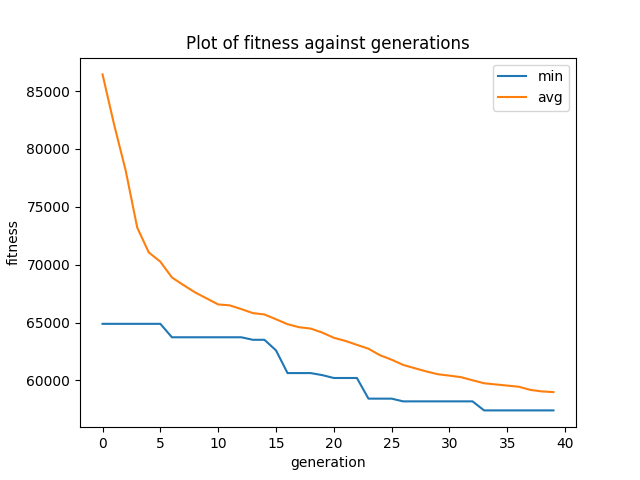
\includegraphics[width=1\linewidth]{images/tsp_fps_tn_gen.png}
      \caption{TSP Single run on 40 generations}
      \label{fig:tsp_fps_tn_sub1}
    \end{subfigure}%
    \begin{subfigure}{.5\textwidth}
      \centering
      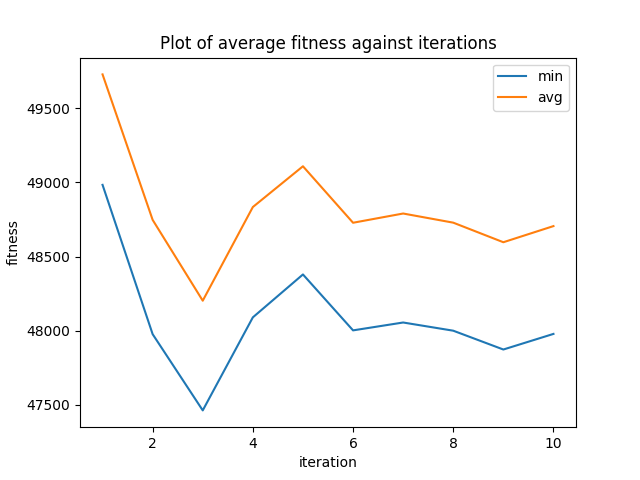
\includegraphics[width=1\linewidth]{images/tsp_fps_tn_itr.png}
      \caption{TSP 10 runs on 1000 generations}
      \label{fig:tsp_fps_tn_sub2}
    \end{subfigure}
    \caption{Note: Fitness is the distance}
    \label{fig:tsp_fps_tn}
  \end{figure}

  As we can our second run was the best one out of the 10.

  \begin{figure}[H]
    \centering
    \textbf{Fitness Proportional Scheme and Binary Tournament Selection Scheme}
    \begin{subfigure}{.5\textwidth}
      \centering
      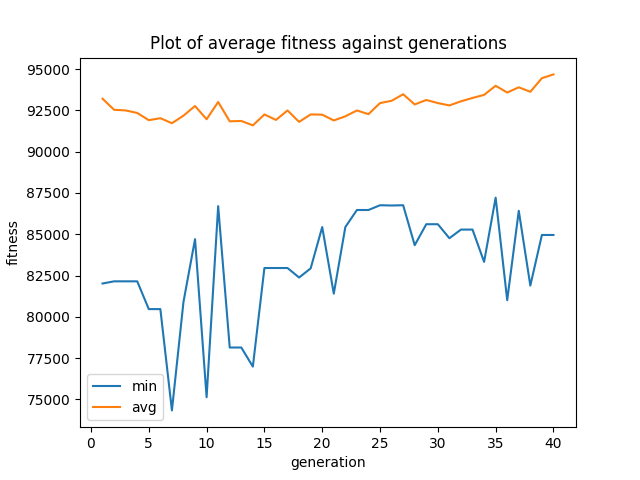
\includegraphics[width=1\linewidth]{images/tsp_fps_bt_gen.png}
      \caption{TSP Single run on 40 generations}
      \label{fig:tsp_fps_bt_sub1}
    \end{subfigure}%
    \begin{subfigure}{.5\textwidth}
      \centering
      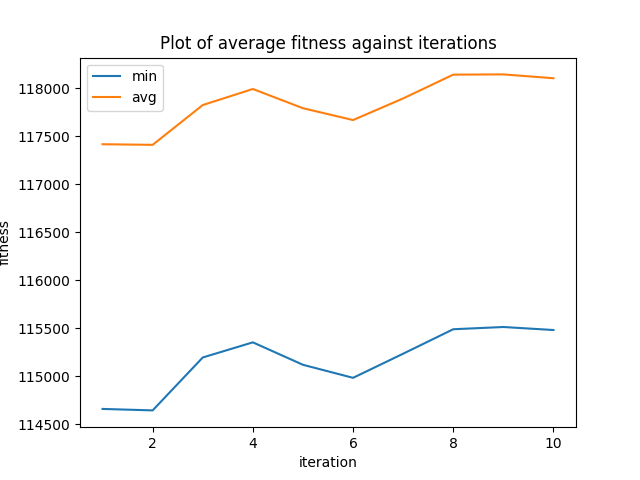
\includegraphics[width=1\linewidth]{images/tsp_fps_bt_itr.png}
      \caption{TSP 10 runs on 1000 generations}
      \label{fig:tsp_fps_bt_sub2}
    \end{subfigure}
    \caption{Note: Fitness is the distance}
    \label{fig:tsp_fps_bt}
  \end{figure}

  \begin{figure}[H]
    \centering
    \textbf{Fitness Proportional Scheme and Random Selection Scheme}
    \begin{subfigure}{.5\textwidth}
      \centering
      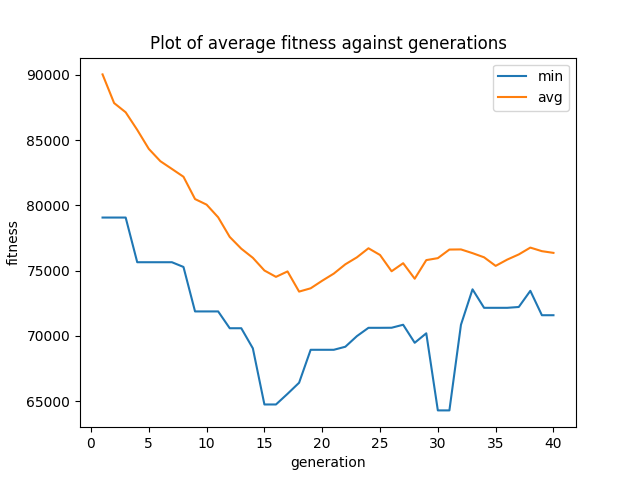
\includegraphics[width=1\linewidth]{images/tsp_fps_rd_gen.png}
      \caption{TSP Single run on 40 generations}
      \label{fig:tsp_fps_rd_sub1}
    \end{subfigure}%
    \begin{subfigure}{.5\textwidth}
      \centering
      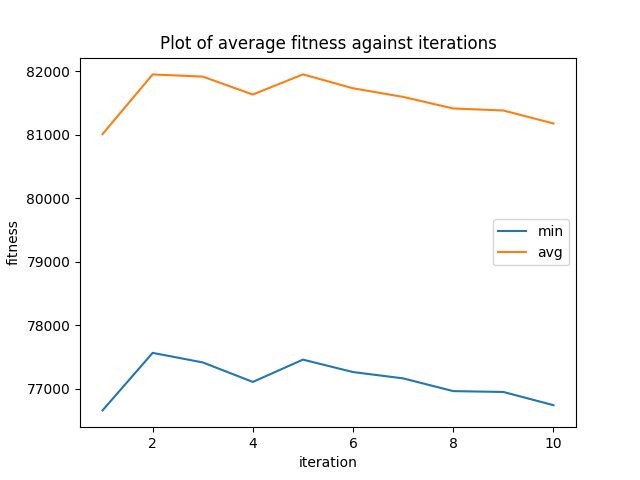
\includegraphics[width=1\linewidth]{images/tsp_fps_rd_itr.png}
      \caption{TSP 10 runs on 1000 generations}
      \label{fig:tsp_fps_rd_sub2}
    \end{subfigure}
    \caption{Note: Fitness is the distance}
    \label{fig:tsp_fps_rd}
  \end{figure}

  \begin{figure}[H]
    \centering
    \textbf{Fitness Proportional Scheme and Rank Based Selection Scheme}
    \begin{subfigure}{.5\textwidth}
      \centering
      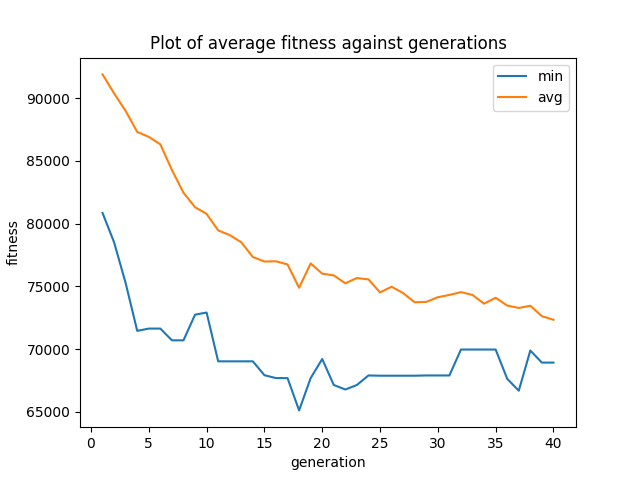
\includegraphics[width=1\linewidth]{images/tsp_fps_rbs_gen.png}
      \caption{TSP Single run on 40 generations}
      \label{fig:tsp_fps_rbs_sub1}
    \end{subfigure}%
    \begin{subfigure}{.5\textwidth}
      \centering
      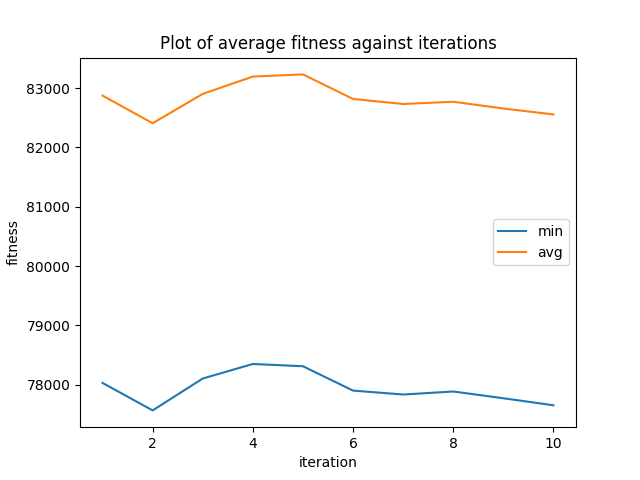
\includegraphics[width=1\linewidth]{images/tsp_fps_rbs_itr.png}
      \caption{TSP 10 runs on 1000 generations}
      \label{fig:tsp_fps_rbs_sub2}
    \end{subfigure}
    \caption{Note: Fitness is the distance}
    \label{fig:tsp_fps_rbs}
  \end{figure}

  \begin{figure}[H]
    \centering
    \textbf{Rank Based Selection and Truncation}
    \begin{subfigure}{.5\textwidth}
      \centering
      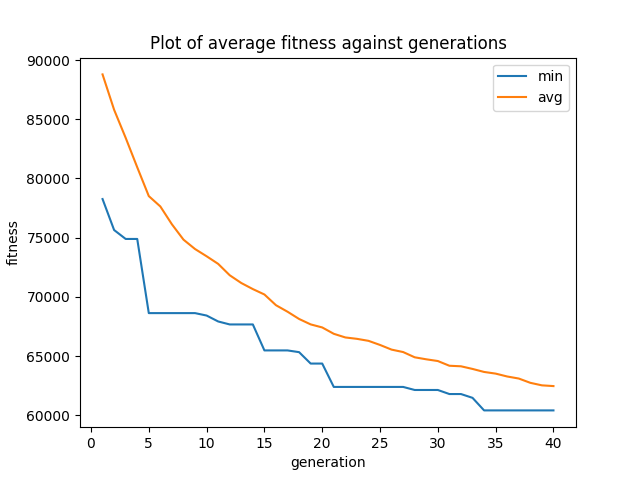
\includegraphics[width=1\linewidth]{images/tsp_rbs_tn_gen.png}
      \caption{TSP Single run on 40 generations}
      \label{fig:tsp_rbs_tn_sub1}
    \end{subfigure}%
    \begin{subfigure}{.5\textwidth}
      \centering
      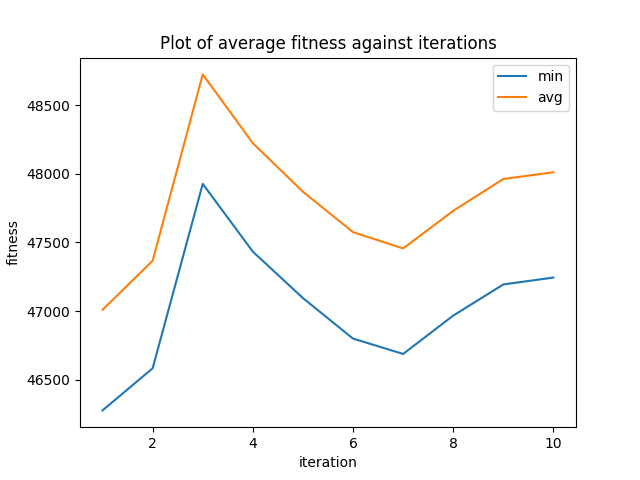
\includegraphics[width=1\linewidth]{images/tsp_rbs_tn_itr.png}
      \caption{TSP 10 runs on 1000 generations}
      \label{fig:tsp_rbs_tn_sub2}
    \end{subfigure}
    \caption{Note: Fitness is the distance}
    \label{fig:tsp_rbs_tn}
  \end{figure}

  \titledquestion{Knapsack Problem}[H]

  \newpage
  \begin{figure}[H]
    \centering
    \textbf{Binary Tournament and Truncation}
    \begin{subfigure}{.5\textwidth}
      \centering
      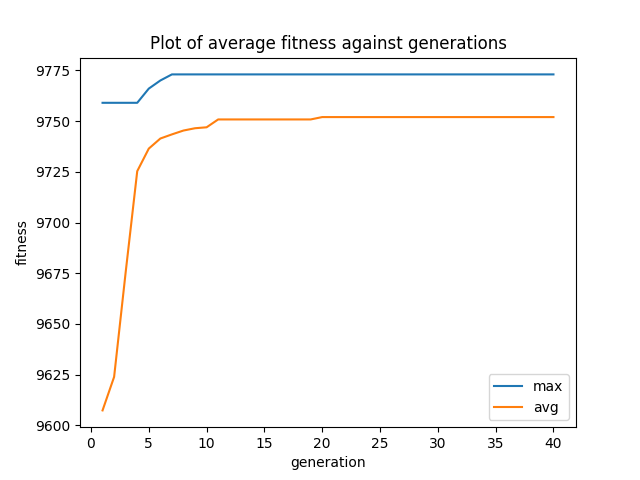
\includegraphics[width=1\linewidth]{images/ks_bt_tn_gen.png}
      \caption{TSP Single run on 40 generations}
      \label{fig:ks_bt_tn_sub1}
    \end{subfigure}%
    \begin{subfigure}{.5\textwidth}
      \centering
      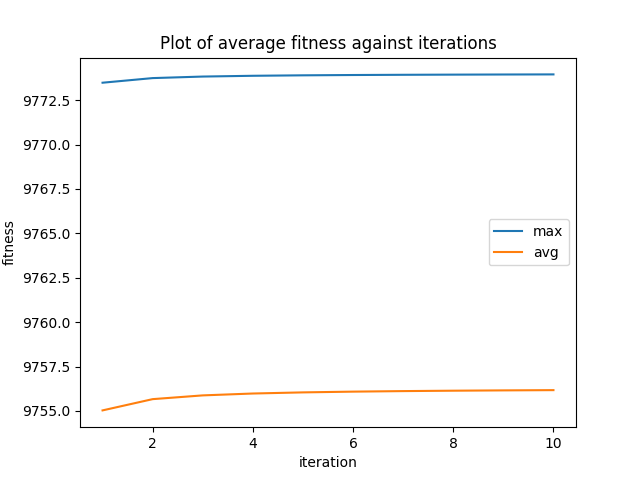
\includegraphics[width=1\linewidth]{images/ks_bt_tn_itr.png}
      \caption{TSP 10 runs on 1000 generations}
      \label{fig:ks_bt_tn_sub2}
    \end{subfigure}
    \caption{Note: Fitness is the distance}
    \label{fig:ks_bt_tn}
  \end{figure}

  \begin{figure}[H]
    \centering
    \textbf{Binary Tournament and Rank Based Selection Scheme}
    \begin{subfigure}{.5\textwidth}
      \centering
      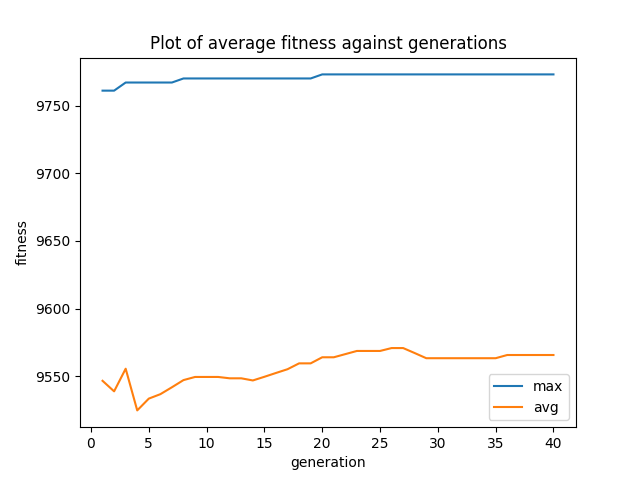
\includegraphics[width=1\linewidth]{images/ks_bt_rbs_gen.png}
      \caption{TSP Single run on 40 generations}
      \label{fig:ks_bt_rbs_sub1}
    \end{subfigure}%
    \begin{subfigure}{.5\textwidth}
      \centering
      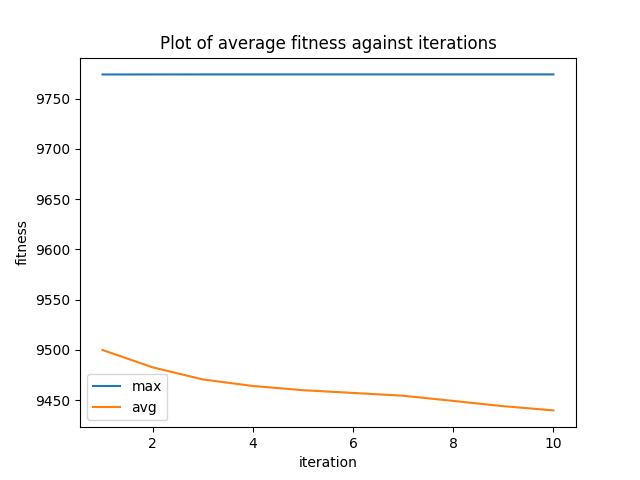
\includegraphics[width=1\linewidth]{images/ks_bt_rbs_itr.png}
      \caption{TSP 10 runs on 1000 generations}
      \label{fig:ks_bt_rbs_sub2}
    \end{subfigure}
    \caption{Note: Fitness is the distance}
    \label{fig:ks_bt_rbs}
  \end{figure}

  \titledquestion{Graph Coloring Problem}[H]
\end{questions}

\end{document}